\documentclass[tikz,border=12pt]{standalone}
\usepackage[T1]{fontenc}
\usepackage{helvet}
\renewcommand{\familydefault}{\sfdefault}
\usepackage{amsmath}
\usetikzlibrary{arrows.meta, fit, backgrounds, positioning, calc, shapes.geometric}

% Semantic palette, shared across all method figures. Color encodes role:
%   blue   = BM25 / lexical step
%   red    = LLM step (absent here, used in the hybrid and llm figures)
%   amber  = document data and stores (catalog, trees, a document)
%   green  = retrieved units and final output (leaves, candidates, passages)
%   gray   = query input
% Muted fills with darker same-hue borders keep it professional, not childish.
\definecolor{queryfill}{HTML}{ECEFF2}   % gray, input
\definecolor{queryborder}{HTML}{8A96A3}
\definecolor{bm25fill}{HTML}{E2ECF7}     % blue, BM25 step
\definecolor{bm25border}{HTML}{3C6CA6}
\definecolor{llmfill}{HTML}{F7E4E4}      % red, LLM step (reserved for other figures)
\definecolor{llmborder}{HTML}{BE4F4F}
\definecolor{corpusfill}{HTML}{FBF0D5}   % amber, document data and stores
\definecolor{corpusborder}{HTML}{CFA23E}
\definecolor{outfill}{HTML}{E7F4E7}      % green, retrieved units and output
\definecolor{outborder}{HTML}{59A05B}
\definecolor{poolfill}{HTML}{F1F9F1}
\definecolor{regfill}{HTML}{F6F8FB}
\definecolor{regborder}{HTML}{C4CDD6}
\definecolor{darkline}{HTML}{333333}
\definecolor{subtext}{HTML}{5A5A5A}

\tikzset{
  card/.style={rectangle, rounded corners=5pt, align=center, draw=darkline,
               line width=0.8pt, minimum height=1.2cm, font=\small},
  query/.style={card, fill=queryfill, draw=queryborder, minimum width=2.0cm},
  proc/.style={card, fill=bm25fill, draw=bm25border, minimum width=2.9cm},
  result/.style={card, fill=outfill, draw=outborder, minimum width=2.2cm},
  docbox/.style={card, fill=corpusfill, draw=corpusborder, minimum width=2.2cm},
  tnode/.style={rectangle, rounded corners=4pt, draw=bm25border, fill=bm25fill,
                line width=0.8pt, minimum width=1.8cm, minimum height=0.8cm, font=\scriptsize},
  leaf/.style={rectangle, rounded corners=3pt, draw=outborder, fill=outfill,
               line width=0.8pt, minimum width=1.05cm, minimum height=0.82cm, font=\scriptsize},
  db/.style={cylinder, shape border rotate=90, aspect=0.28, draw=corpusborder,
             fill=corpusfill, line width=0.8pt, minimum width=1.75cm,
             minimum height=1.05cm, font=\scriptsize, align=center, inner sep=1pt},
  region/.style={rounded corners=12pt, fill=regfill, draw=regborder, line width=0.8pt},
  pooldash/.style={draw=outborder, dashed, rounded corners=8pt, fill=poolfill,
                   line width=0.85pt},
  regtitle/.style={font=\small\bfseries, text=darkline},
  note/.style={font=\scriptsize\itshape, text=subtext, align=center},
  flow/.style={-{Latex[length=2.2mm]}, line width=0.85pt, draw=darkline},
  feed/.style={-{Latex[length=1.9mm]}, line width=0.7pt, draw=corpusborder},
  branch/.style={-{Latex[length=1.7mm]}, line width=0.65pt, draw=darkline},
}

\def\inlen{0.9cm}    % input/output connector
\def\stagegap{1.7cm} % between stages, wide enough that panels never overlap
\def\intra{0.95cm}   % within a stage
\def\dnode{1.1cm}
\def\nleaf{1.0cm}
\def\nspread{1.35cm}
\def\lspread{0.78cm}
\def\dbdrop{1.1cm}   % cylinder distance below the spine box

\begin{document}
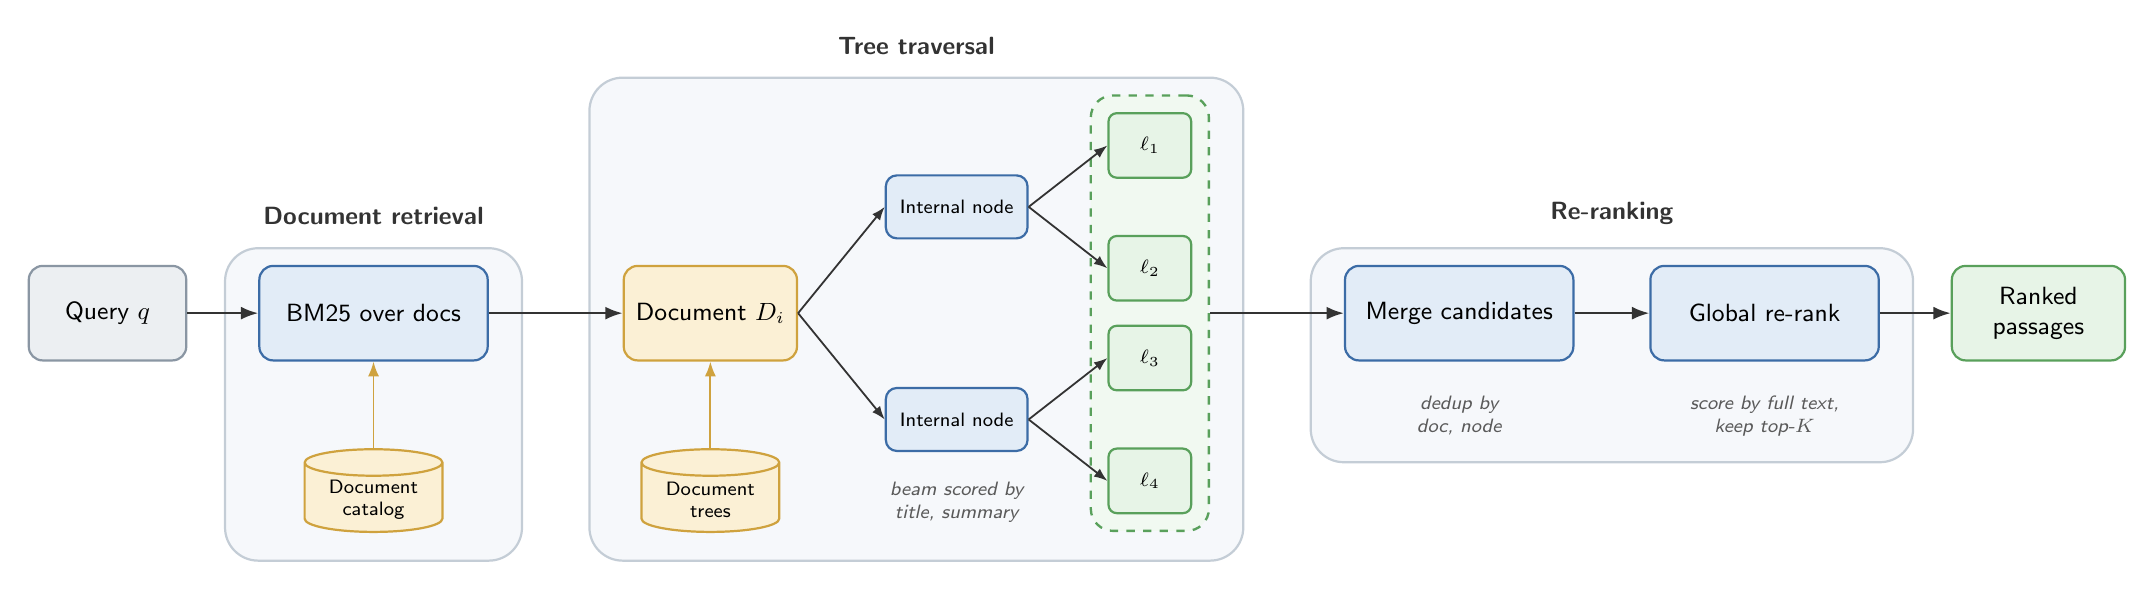
\begin{tikzpicture}

% Input (outside the phases)
\node[query] (query) {Query $q$};

% Stage 1: Document retrieval
\node[proc, right=\inlen of query] (bm25) {BM25 over docs};
\node[db, below=\dbdrop of bm25] (catalog) {Document\\catalog};

% Stage 2: Tree traversal
\node[docbox, right=\stagegap of bm25] (doc) {Document $D_i$};
\node[db, below=\dbdrop of doc] (trees) {Document\\trees};
\node[tnode, right=\dnode of doc, yshift=\nspread] (n1) {Internal node};
\node[tnode, right=\dnode of doc, yshift=-\nspread] (n2) {Internal node};
\node[leaf, right=\nleaf of n1, yshift=\lspread]  (l1) {$\ell_1$};
\node[leaf, right=\nleaf of n1, yshift=-\lspread] (l2) {$\ell_2$};
\node[leaf, right=\nleaf of n2, yshift=\lspread]  (l3) {$\ell_3$};
\node[leaf, right=\nleaf of n2, yshift=-\lspread] (l4) {$\ell_4$};
\node[pooldash, fit=(l1)(l2)(l3)(l4), inner sep=6pt] (pool) {};
\foreach \n/\t in {l1/\ell_1, l2/\ell_2, l3/\ell_3, l4/\ell_4} {
  \node[leaf] at (\n) {$\t$};
}

% Stage 3: Re-ranking
\node[proc, right=\stagegap of pool] (merge) {Merge candidates};
\node[proc, right=\intra of merge] (rerank) {Global re-rank};

% Output (outside the phases)
\node[result, right=\inlen of rerank] (sources) {Ranked\\passages};

% Notes. The data-source detail and the pool re-ranking detail live in the
% caption, so no deep notes drag the panel band downward.
\node[note] (nnote) at ($(n2)+(0,-1.05)$) {beam scored by\\title, summary};
\node[note, below=0.32cm of merge] (mergenote) {dedup by\\doc, node};
\node[note, below=0.32cm of rerank] (reranknote) {score by full text,\\keep top-$K$};

% Phase panels, equal height, input/output excluded
\begin{scope}[on background layer]
  % Panels share a common bottom baseline. Each hugs its own content upward,
  % so the tree panel is taller without forcing dead space on the others.
  \coordinate (bandB) at ($(trees.south)+(0,-0.14)$);
  \node[region, inner xsep=12pt, inner ysep=6pt,
        fit=(bm25)(catalog)(bm25|-bandB)] (reg1) {};
  \node[region, inner xsep=12pt, inner ysep=6pt,
        fit=(doc)(trees)(n1)(n2)(nnote)(pool)(doc|-bandB)] (reg2) {};
  \node[region, inner xsep=12pt, inner ysep=6pt,
        fit=(merge)(rerank)(mergenote)(reranknote)] (reg3) {};
\end{scope}
\node[regtitle, anchor=south] at ($(reg1.north)+(0,0.16)$) {Document retrieval};
\node[regtitle, anchor=south] at ($(reg2.north)+(0,0.16)$) {Tree traversal};
\node[regtitle, anchor=south] at ($(reg3.north)+(0,0.16)$) {Re-ranking};

% Flow
\draw[flow] (query) -- (bm25);
\draw[flow] (bm25.east) -- (doc.west);
\draw[feed] (catalog.north) -- (bm25.south);
\draw[feed] (trees.north) -- (doc.south);
\draw[branch] (doc.east) -- (n1.west);
\draw[branch] (doc.east) -- (n2.west);
\draw[branch] (n1.east) -- (l1.west);
\draw[branch] (n1.east) -- (l2.west);
\draw[branch] (n2.east) -- (l3.west);
\draw[branch] (n2.east) -- (l4.west);
\draw[flow] (pool.east) -- (merge.west);
\draw[flow] (merge) -- (rerank);
\draw[flow] (rerank) -- (sources);

\end{tikzpicture}
\end{document}
